% =====================================================================
%  Farm Invoice Manager - Project Report
%  CSC2210: Object Oriented Programming 2 (Fall 2025-2026)
%
%  Build:  latexmk -pdf main.tex      (or pdflatex main.tex twice)
% =====================================================================
\documentclass[12pt,a4paper]{article}

\usepackage[T1]{fontenc}
\usepackage{mathptmx}
\usepackage[margin=1in]{geometry}
\usepackage{graphicx}
\usepackage{array}
\usepackage{longtable}
\usepackage{tabularx}
\usepackage[table]{xcolor}
\usepackage{enumitem}
\usepackage{listings}
\usepackage{titlesec}
\usepackage{float}
\usepackage{caption}
\usepackage[hidelinks]{hyperref}

\graphicspath{{figures/}}

\definecolor{navy}{RGB}{0,32,96}
\definecolor{codebg}{RGB}{246,246,246}
\newcolumntype{C}[1]{>{\centering\arraybackslash}p{#1}}
\newcolumntype{L}[1]{>{\raggedright\arraybackslash}p{#1}}
\newcommand{\head}[1]{\cellcolor{navy}\textcolor{white}{\textbf{#1}}}

% chapter-like headings: "Chapter 01: Introduction"
\titleformat{\section}{\large\bfseries}{}{0pt}{}
\titlespacing*{\section}{0pt}{14pt}{8pt}
\titleformat{\subsection}{\normalsize\bfseries}{}{0pt}{}
\setcounter{secnumdepth}{0}

\setlist{nosep}
\setlength{\parindent}{0pt}
\setlength{\parskip}{6pt}

\lstset{
  language=SQL,
  basicstyle=\ttfamily\footnotesize,
  keywordstyle=\bfseries\color{navy},
  backgroundcolor=\color{codebg},
  frame=single, rulecolor=\color{gray!50},
  breaklines=true, columns=fullflexible,
  aboveskip=4pt, belowskip=6pt,
  morekeywords={NVARCHAR,BIT,IDENTITY,GETDATE,ISNULL,TOP}
}

% "Form Name / Purpose" block with one screenshot
\newcommand{\screen}[3]{%
  \begin{minipage}{\textwidth}
  \textbf{Form Name:} #1\\
  \textbf{Purpose:} #2\par\vspace{4pt}
  \centering\includegraphics[width=0.78\textwidth,height=0.36\textheight,keepaspectratio]{screens/#3}
  \end{minipage}\par\vspace{14pt}}

\begin{document}

% =====================================================================
%  COVER PAGE
% =====================================================================
\begin{titlepage}
\centering
\vspace*{-1.2cm}
\includegraphics[width=2.8cm]{aiub_logo.png}\par\vspace{8pt}
{\large\bfseries AMERICAN INTERNATIONAL UNIVERSITY--BANGLADESH (AIUB)}\par\vspace{6pt}
{\bfseries Dept. of Computer Science\\ Faculty of Science and Technology}\par\vspace{10pt}
{\bfseries CSC2210: OBJECT ORIENTED PROGRAMMING 2}\par\vspace{10pt}
{\bfseries Fall 2025-2026\\[4pt] Section: [G]\\[4pt] Group No: 09}\par\vspace{12pt}
{\large\bfseries Project Report On}\par\vspace{6pt}
{\Large\bfseries\itshape Project name [ Farm Invoice Manager]}\par\vspace{8pt}
{\bfseries Supervised By\\[4pt] Md. Hasibul Hasan}\par\vspace{14pt}
{\large\bfseries Submitted By:} {\bfseries MAHMMOD, MD. SHAFI}\par\vspace{4pt}

\renewcommand{\arraystretch}{1.25}
\begin{tabular}{|L{4.4cm}|C{1.9cm}|C{1.6cm}|C{1.5cm}|C{1.3cm}|L{1.6cm}|}
\hline
\multicolumn{4}{|c|}{Name} & \multicolumn{2}{c|}{ID} \\ \hline
\multicolumn{4}{|l|}{\textbf{TASNIM, JARIN}} & \multicolumn{2}{l|}{\textbf{23-50749-1}} \\ \hline
\multicolumn{4}{|l|}{\textbf{MAHMMOD, MD. SHAFI}} & \multicolumn{2}{l|}{\textbf{23-54122-3}} \\ \hline
\multicolumn{4}{|l|}{\textbf{RISHAD, NAJIAT ISLAM}} & \multicolumn{2}{l|}{\textbf{23-55218-3}} \\ \hline
\multicolumn{6}{|c|}{\small\textbf{Obtained Marks for CO2 and CO3 (Description given in the following page)}} \\ \hline
\head{\small Assessment Criteria} & \head{\small Not Attended/ Incorrect (0)} & \head{\small Inadequate (1-2)} & \head{\small Average (3)} & \head{\small Good (4)} & \head{\small Excellent (5)} \\ \hline
\small\textbf{Evaluation Criteria (CO2)} & \small\textbf{Total =} & \multicolumn{2}{l|}{\small\textbf{Evaluation Criteria (CO3)}} & \multicolumn{2}{l|}{\small\textbf{Total =}} \\ \hline
\small Requirement fulfillment & & \multicolumn{2}{l|}{\small Organization of the application} & \multicolumn{2}{l|}{} \\ \hline
\small Validation & & \multicolumn{2}{L{3.1cm}|}{\small Representation and Integration of Database} & \multicolumn{2}{l|}{} \\ \hline
\small Verification & & \multicolumn{2}{l|}{\small Graphical User Interface} & \multicolumn{2}{l|}{} \\ \hline
\end{tabular}
\end{titlepage}

% =====================================================================
%  RUBRIC PAGES
% =====================================================================
{\footnotesize
\renewcommand{\arraystretch}{1.2}
\begin{longtable}{|L{1.9cm}|L{2.3cm}|L{2.3cm}|L{2.3cm}|L{2.3cm}|L{2.3cm}|}
\hline
\multicolumn{6}{|L{15.0cm}|}{\textbf{CO2:} Display and verify the mean of a real-life Project using the concepts of C\# Graphical User Interface based environment with database integration to depict a desktop-based application.} \\ \hline
\head{Assessment Criteria} & \head{Not Attended/ Incorrect (0)} & \head{Inadequate (1-2)} & \head{Average (3)} & \head{Good (4)} & \head{Excellent (5)} \\ \hline
\textbf{Evaluation Criteria} & \multicolumn{5}{c|}{\textbf{Evaluation Definition}} \\ \hline
\endhead
Requirement fulfillment &
Fails to demonstrate any understanding of real-life scenario-based project development or functional requirement identification. There is no attempt to depict a project or identify functional requirements accurately. &
Demonstrates limited understanding of real-life scenario-based project development and functional requirement identification. The project depicted lacks coherence or relevance to real-life scenarios, and functional requirements are inaccurately identified or insufficiently described. &
Presents a basic depiction of a real-life scenario-based project and identifies some functional requirements. However, the project lacks depth or complexity, and some functional requirements may be vaguely defined or missing key details. &
Effectively demonstrates a realistic scenario-based project and accurately identifies most functional requirements. The project is well-developed with appropriate complexity, and functional requirements are clearly articulated with relevant details. &
Exhibits an exceptional understanding of real-life scenario-based project development and accurately identifies all functional requirements. The project is meticulously developed with thorough attention to detail, reflecting a comprehensive understanding of Object-Oriented Programming project development activities. \\ \hline
Validation &
Fails to demonstrate any understanding or implementation of validation forms in their system. There is no attempt to deal with data validation, and validation requirements are completely ignored or incorrectly applied. &
Demonstrates limited understanding of validation forms and data validation techniques. While some attempt may be made to implement validation, it is incomplete or poorly executed, leading to inadequate handling of data validation. &
Shows a basic understanding of validation forms and data validation techniques. They attempt to implement validation, but some aspects may be missing or incorrectly implemented, resulting in partial or inconsistent handling of data validation. &
Effectively demonstrates the use of validation forms and implements data validation techniques. Validation is mostly accurate and comprehensive, ensuring the proper handling of data input and verification in the system. &
Exhibits an exceptional understanding and implementation of validation forms and data validation techniques. Validation is meticulously implemented with thorough attention to detail, ensuring robust data validation procedures and contributing to the overall reliability and integrity of the system. \\ \hline
Verification &
Fails to demonstrate any attempt to verify the system data or functional requirements. There is no evidence of understanding or implementation of verification processes, and data flow is not considered. &
Demonstrates limited understanding of verification processes and data flow in the system. Verification attempts are incomplete or inaccurate, and there is insufficient consideration given to ensuring data integrity and functionality. &
Shows a basic understanding of verification processes and attempts to verify system data. However, verification efforts may be inconsistent or lack thoroughness, and there may be gaps in ensuring proper functional requirements and data flow. &
Identifies and verifies system data, ensuring proper functional requirements are met. Verification efforts are mostly accurate and thorough, with attention to ensuring data integrity and appropriate data flow within the system. &
Exhibits an exceptional understanding of verification processes and meticulously verifies system data. Verification efforts are comprehensive and precise, with a keen focus on ensuring all functional requirements are met and maintaining proper data flow throughout the system. \\ \hline
\end{longtable}

\begin{longtable}{|L{1.9cm}|L{2.3cm}|L{2.3cm}|L{2.3cm}|L{2.3cm}|L{2.3cm}|}
\hline
\multicolumn{6}{|L{15.0cm}|}{\textbf{CO3:} Prepare and Explain a real life desktop based application synthesizing several component of C\# along with development tools to adhere the given requirements.} \\ \hline
\head{Assessment Criteria} & \head{Not Attended/ Incorrect (0)} & \head{Inadequate (1-2)} & \head{Average (3)} & \head{Good (4)} & \head{Excellent (5)} \\ \hline
\textbf{Evaluation Criteria} & \multicolumn{5}{c|}{\textbf{Evaluation Definition}} \\ \hline
\endhead
Organization of the application &
Fails to identify any suitable real time application or requirements for project development activities related to OOP. &
Limited understanding about the project scopes and scenarios or identification of functional requirements. &
Lacks depth or relevance to OOP project development activities and may contain inaccuracies. Real-life scenarios are mentioned, but the discussion lacks depth or clarity. &
Consider and integrate the idea of several core aspects of the project along with relevance to real-life scenarios. Demonstrating a solid understanding of the application presentation. &
Generalize and exhibits an exceptional understanding of project preparation according to real-life scenarios. Also contains proper and insightful identification of the system which is comprehensive and precise. \\ \hline
Representation and Integration of Database &
Fails to identify and present any understanding or implementation of database. Also failed to integrate the data with the project itself. &
Limited understanding of the database concepts or their proper way of using in a real time project. While some attempt may be made to implement but it is incomplete or poorly executed, leading to inadequate design. &
Lacks depth or relevance to database integration with the application. Shows a basic understanding but some aspects may be missing or incorrectly implemented, resulting in partial or inconsistency. May lack proper normalization. &
Integrate the database with the forms properly and implements it with proper validation which is mostly accurate and comprehensive, ensuring the proper handling of data input and verification along with general normalization. &
Exhibits an exceptional understanding and implementation of database ensuring attention to detail, and robust data manipulation procedures and contributing to the overall clarity. \\ \hline
Graphical User Interface &
Fails to present or prepare GUI based application interfaces. There is no evidence of creating or integrating such things according to their usefulness. &
Limited understanding of graphical user interfaces. Lack of design knowledge. Very poor attempt to make such things which are currently obsolete or can't be identified as coherent. &
Shows a basic understanding of creating user interfaces. Most of them are interconnected but maybe some of them lack it. However, most of it can be described as user friendly. &
Effectively identifies and meet the consider the simplicity. Design related works are mostly accurate and taken proper attention to ensuring a user-friendly coherent system. &
Exhibits an exceptional work design following a high standard of simple and elegant work. Several controls and mechanism has been organized in a preferred way according to the coherent usage. \\ \hline
\end{longtable}
}

\clearpage
% =====================================================================
%  TABLE OF CONTENTS
% =====================================================================
\textbf{\large Table of Contents:}\hfill\textbf{Page no}

\vspace{4pt}
\renewcommand{\arraystretch}{1.4}
\begin{tabularx}{\textwidth}{@{}l X r@{}}
1. & Chapter 01 (Introduction)\dotfill & \pageref{ch:intro} \\
2. & Chapter 02 (User Story)\dotfill & \pageref{ch:story} \\
3. & Chapter 03a (ER Diagram)\dotfill & \pageref{ch:er} \\
4. & Chapter 03b (SQL Queries)\dotfill & \pageref{ch:sql} \\
5. & Chapter 04 (Screenshots)\dotfill & \pageref{ch:screens} \\
\end{tabularx}

% =====================================================================
\section{Chapter 01: Introduction}\label{ch:intro}

The \textbf{Farm Invoice Manager -- Billing Management System} is a desktop-based application developed using \textbf{C\# Windows Forms} and \textbf{SQL Server} to manage billing, sales, products, customers and users in a farm-based business. The main goal of the system is to simplify and automate the manual invoice and sales management process, reducing errors and improving productivity.

The system provides a \textbf{secure login} with role-based access for \textbf{Admin} and \textbf{Employee}. Admin users can manage users, products and customers and view sales reports, while employees can make sales, view customers and see their own information. The application supports \textbf{product management}, \textbf{customer management}, \textbf{invoice generation}, \textbf{sales reporting} and \textbf{printable invoices}. Features such as \textbf{password recovery}, \textbf{username and password reset}, \textbf{premium membership}, \textbf{date-wise sales reports} and \textbf{graphical sales analysis} improve usability and decision-making.

All input fields are checked while the user types, all database queries use parameters, and saving an invoice (invoice details, items and stock update) is done in one transaction, so the data stays correct. With a user-friendly interface and structured data handling, the Farm Invoice Manager helps farm businesses keep accurate records, track inventory, manage customers and produce reliable financial reports. Overall, this project shows the use of object-oriented programming, database connectivity and real-world business logic in a desktop application.

% =====================================================================
\section{Chapter 02: User Story}\label{ch:story}

The Farm Invoice Manager -- Billing Management System is designed for two user roles: \textbf{Admin} and \textbf{Employee}. Each role has its own responsibilities and access permissions to keep farm billing and sales safe and efficient. Below is a short overview of how each user works with the system.

\subsection{As an Admin}
\begin{itemize}
\item Log in securely to the admin dashboard using a username (or User ID) and password.
\item Add, update, search or remove system users and manage their personal and login information.
\item Add new farm products, update product details such as name, category, stock and unit price, and remove products that are not used in any invoice.
\item View, search and delete premium customers.
\item Create sales invoices with a discount and add new premium customers during a sale.
\item View, print and delete invoices.
\item View sales reports with date-wise filtering, customer search and a sales chart.
\item View personal information and reset own username and password.
\item Log out safely to protect system data.
\end{itemize}

\subsection{As an Employee}
\begin{itemize}
\item Log in securely to the employee dashboard using authorized credentials.
\item View personal information and account details.
\item View and search premium customers.
\item Add new premium customers during sales transactions.
\item Create sales invoices by selecting products and entering quantities.
\item View sales reports and print invoices for customers.
\item Reset own username and password for security purposes.
\item Log out safely after completing work.
\end{itemize}

% =====================================================================
\section{Chapter 03a: ER Diagram}\label{ch:er}

\begin{figure}[H]
\centering
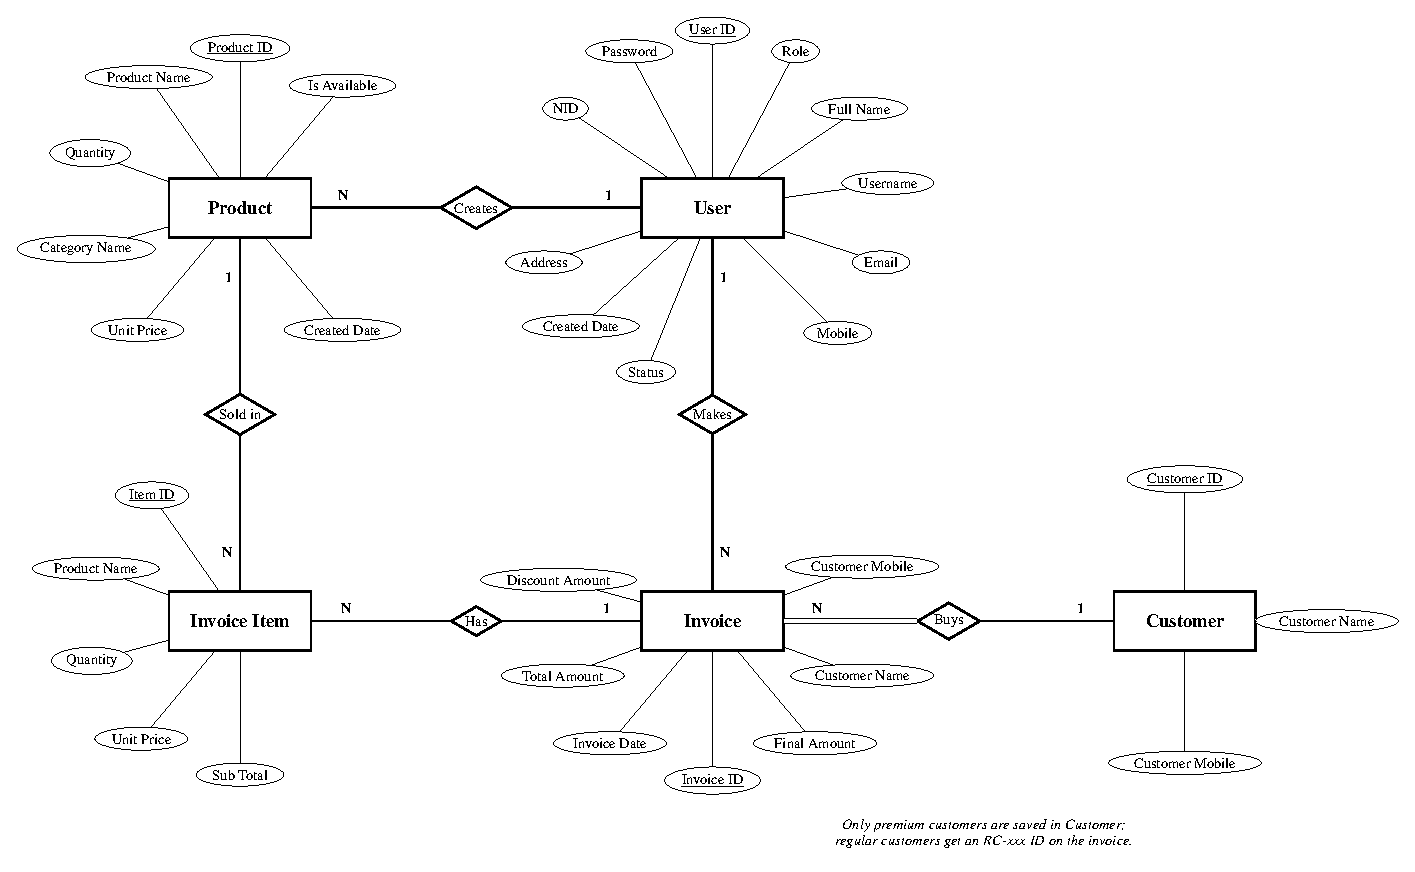
\includegraphics[width=\textwidth]{er_diagram.pdf}
\caption*{ER Diagram of the Farm Invoice Manager database}
\end{figure}

\subsection{Explanation of Entities and Relationships:}

\textbf{UserInfo} (stores admin and employee information)
\begin{itemize}
\item USER\_ID (Primary Key, A-xxx for admin, E-xxx for employee)
\item ROLE (admin / employee)
\item FULL\_NAME, USERNAME, EMAIL, MOBILE, PASSWORD, NID, ADDRESS
\item CREATED\_DATE
\item STATUS (1 = Active, 0 = Inactive)
\end{itemize}

\textbf{CustomerInfo} (stores premium customer details)
\begin{itemize}
\item CUSTOMER\_ID (Primary Key, PC-xxx)
\item CUSTOMER\_NAME
\item CUSTOMER\_MOBILE
\end{itemize}

\textbf{ProductInfo} (stores product and inventory details)
\begin{itemize}
\item PRODUCT\_ID (Primary Key, FIM-xxx)
\item PRODUCT\_NAME, QUANTITY (stock), CATEGORY\_NAME, UNITPRICE
\item CREATED\_DATE, IS\_AVAILABLE
\item CREATED\_BY\_USER\_ID (Foreign Key $\rightarrow$ UserInfo)
\end{itemize}

\textbf{InvoiceDetails} (stores the summary of each invoice)
\begin{itemize}
\item INVOICE\_ID (Primary Key, INV-xxx)
\item USER\_ID (Foreign Key $\rightarrow$ UserInfo, the user who made the sale)
\item CUSTOMER\_ID (PC-xxx for a premium customer, RC-xxx for a regular customer)
\item CUSTOMER\_NAME, CUSTOMER\_MOBILE (stored on the invoice for quick display)
\item TOTAL\_AMOUNT, DISCOUNT\_AMOUNT, FINAL\_AMOUNT
\item INVOICE\_DATE
\end{itemize}

\textbf{InvoiceItems} (stores the products of each invoice)
\begin{itemize}
\item INVOICE\_ITEM\_ID (Primary Key, auto number)
\item INVOICE\_ID (refers to InvoiceDetails)
\item PRODUCT\_ID (Foreign Key $\rightarrow$ ProductInfo)
\item PRODUCT\_NAME, QUANTITY, UNIT\_PRICE, SUB\_TOTAL
\end{itemize}

\textbf{Relationships}
\begin{itemize}
\item One \textbf{User} creates many \textbf{Products} (1 : N).
\item One \textbf{User} makes many \textbf{Invoices} (1 : N).
\item One \textbf{Invoice} has many \textbf{Invoice Items} (1 : N).
\item One \textbf{Product} can be sold in many \textbf{Invoice Items} (1 : N).
\item One premium \textbf{Customer} can buy many times, so one customer has many \textbf{Invoices} (1 : N). Regular customers are not saved in CustomerInfo, so not every invoice has a customer record.
\end{itemize}

% =====================================================================
\section{Chapter 03b: SQL Queries}\label{ch:sql}

\subsection{1. Database Creation}
The database stores all information about users, customers, products, invoices and sales.

\textbf{Database Name:} FarmInvoiceManager. The complete script (database, tables and sample data) is \texttt{Database/FarmInvoiceManager.sql}.
\begin{lstlisting}
CREATE DATABASE FarmInvoiceManager;
GO
USE FarmInvoiceManager;
\end{lstlisting}

\subsection{2. Table Creation}
Five tables represent the main entities of the system:
\begin{itemize}
\item \textbf{UserInfo} -- stores admin and employee information
\item \textbf{CustomerInfo} -- stores premium customer details
\item \textbf{ProductInfo} -- stores product information
\item \textbf{InvoiceDetails} -- stores invoice summary data
\item \textbf{InvoiceItems} -- stores item-wise invoice details
\end{itemize}

\begin{lstlisting}
CREATE TABLE UserInfo (
    USER_ID       NVARCHAR(10)  NOT NULL PRIMARY KEY,
    ROLE          NVARCHAR(10)  NOT NULL,
    FULL_NAME     NVARCHAR(50)  NOT NULL,
    USERNAME      NVARCHAR(50)  NOT NULL,
    EMAIL         NVARCHAR(50)  NOT NULL,
    MOBILE        NVARCHAR(20)  NOT NULL,
    PASSWORD      NVARCHAR(50)  NOT NULL,
    NID           NVARCHAR(20)  NOT NULL,
    ADDRESS       NVARCHAR(50)  NOT NULL,
    CREATED_DATE  DATE          NOT NULL,
    STATUS        BIT           NOT NULL
);

CREATE TABLE CustomerInfo (
    CUSTOMER_ID      NVARCHAR(10) NOT NULL PRIMARY KEY,
    CUSTOMER_NAME    NVARCHAR(50) NOT NULL,
    CUSTOMER_MOBILE  NVARCHAR(20) NOT NULL
);

CREATE TABLE ProductInfo (
    PRODUCT_ID          NVARCHAR(10) NOT NULL PRIMARY KEY,
    PRODUCT_NAME        NVARCHAR(50) NOT NULL,
    QUANTITY            INT          NOT NULL,
    CATEGORY_NAME       NVARCHAR(50) NOT NULL,
    UNITPRICE           FLOAT        NOT NULL,
    CREATED_DATE        DATE         NOT NULL,
    IS_AVAILABLE        BIT          NOT NULL,
    CREATED_BY_USER_ID  NVARCHAR(10) NOT NULL REFERENCES UserInfo(USER_ID)
);

CREATE TABLE InvoiceDetails (
    INVOICE_ID       NVARCHAR(10)  NOT NULL PRIMARY KEY,
    USER_ID          NVARCHAR(10)  NOT NULL REFERENCES UserInfo(USER_ID),
    CUSTOMER_ID      NVARCHAR(10)  NOT NULL,
    CUSTOMER_NAME    NVARCHAR(50)  NOT NULL,
    CUSTOMER_MOBILE  NVARCHAR(20)  NOT NULL,
    TOTAL_AMOUNT     DECIMAL(10,2) NOT NULL,
    DISCOUNT_AMOUNT  DECIMAL(10,2) NOT NULL,
    FINAL_AMOUNT     DECIMAL(10,2) NOT NULL,
    INVOICE_DATE     DATE          NOT NULL
);

CREATE TABLE InvoiceItems (
    INVOICE_ITEM_ID  INT IDENTITY(1,1) PRIMARY KEY,
    INVOICE_ID       NVARCHAR(10)  NOT NULL,
    PRODUCT_ID       NVARCHAR(10)  NOT NULL REFERENCES ProductInfo(PRODUCT_ID),
    PRODUCT_NAME     NVARCHAR(100) NOT NULL,
    QUANTITY         INT           NOT NULL,
    UNIT_PRICE       DECIMAL(10,2) NOT NULL,
    SUB_TOTAL        DECIMAL(10,2) NOT NULL
);
\end{lstlisting}

\subsection{3. Queries Used in the Application}
All queries are sent with parameters (\texttt{@Name}) through one database class (\texttt{Data/Db.cs}), and the connection string is written only once in \texttt{App.config}. This protects the system from SQL injection. The main queries of each form are given below.

\textbf{FormLogin}
\begin{lstlisting}
SELECT USER_ID, FULL_NAME, ROLE, STATUS FROM UserInfo
WHERE (USERNAME = @User OR USER_ID = @User) AND PASSWORD = @Password;
\end{lstlisting}

\textbf{FormFindPassword}
\begin{lstlisting}
SELECT PASSWORD FROM UserInfo
WHERE USER_ID = @ID AND USERNAME = @Username AND MOBILE = @Mobile;
\end{lstlisting}

\textbf{FormAdminView}
\begin{lstlisting}
SELECT * FROM UserInfo ORDER BY USER_ID;

SELECT * FROM UserInfo
WHERE FULL_NAME LIKE @Search OR USERNAME LIKE @Search OR USER_ID LIKE @Search
ORDER BY USER_ID;

DELETE FROM UserInfo WHERE USER_ID = @ID;
DELETE FROM CustomerInfo WHERE CUSTOMER_ID = @ID;
\end{lstlisting}

\textbf{FormAdminView and FormEmployee (shared: customers and personal information)}
\begin{lstlisting}
SELECT * FROM CustomerInfo ORDER BY CUSTOMER_ID;

SELECT * FROM CustomerInfo WHERE CUSTOMER_MOBILE LIKE @Search ORDER BY CUSTOMER_ID;

SELECT * FROM UserInfo WHERE USER_ID = @ID;
\end{lstlisting}

\textbf{FormAddUser}
\begin{lstlisting}
-- next ID: admins (A-) and employees (E-) share one counter
SELECT ISNULL(MAX(CAST(SUBSTRING(USER_ID, 3, 10) AS INT)), 0)
FROM UserInfo WHERE USER_ID LIKE '[AE]-%';

SELECT COUNT(*) FROM UserInfo WHERE USERNAME = @U;

INSERT INTO UserInfo (USER_ID, ROLE, FULL_NAME, USERNAME, EMAIL, MOBILE,
                      PASSWORD, NID, ADDRESS, CREATED_DATE, STATUS)
VALUES (@ID, @Role, @FullName, @Username, @Email, @Mobile,
        @Password, @NID, @Address, CAST(GETDATE() AS DATE), @Status);
\end{lstlisting}

\textbf{FormEditUser}
\begin{lstlisting}
SELECT * FROM UserInfo WHERE USER_ID = @ID;

SELECT COUNT(*) FROM UserInfo WHERE USERNAME = @U AND USER_ID <> @ID;

UPDATE UserInfo
SET FULL_NAME = @FullName, EMAIL = @Email, USERNAME = @Username,
    PASSWORD = @Password, MOBILE = @Mobile, NID = @NID,
    ADDRESS = @Address, STATUS = @Status
WHERE USER_ID = @ID;
\end{lstlisting}

\textbf{FormReset}
\begin{lstlisting}
SELECT USERNAME, PASSWORD FROM UserInfo WHERE USER_ID = @ID;

UPDATE UserInfo SET USERNAME = @NewUser, PASSWORD = @NewPassword
WHERE USER_ID = @ID AND USERNAME = @OldUser AND PASSWORD = @OldPassword;
\end{lstlisting}

\textbf{FormManageProducts}
\begin{lstlisting}
SELECT * FROM ProductInfo ORDER BY PRODUCT_ID;

SELECT * FROM ProductInfo
WHERE PRODUCT_NAME LIKE @Search OR PRODUCT_ID LIKE @Search
ORDER BY PRODUCT_ID;

DELETE FROM ProductInfo WHERE PRODUCT_ID = @ID;
\end{lstlisting}

\textbf{FormAddProduct}
\begin{lstlisting}
SELECT ISNULL(MAX(CAST(SUBSTRING(PRODUCT_ID, 5, 10) AS INT)), 0)
FROM ProductInfo WHERE PRODUCT_ID LIKE 'FIM-%';

INSERT INTO ProductInfo (PRODUCT_ID, PRODUCT_NAME, QUANTITY, CATEGORY_NAME,
                         UNITPRICE, CREATED_DATE, IS_AVAILABLE, CREATED_BY_USER_ID)
VALUES (@ID, @Name, @Qty, @Category, @Price, @Date, @Available, @CreatedBy);
\end{lstlisting}

\textbf{FormUpdateProduct}
\begin{lstlisting}
SELECT * FROM ProductInfo WHERE PRODUCT_ID = @ID;

UPDATE ProductInfo
SET PRODUCT_NAME = @Name, QUANTITY = @Qty, CATEGORY_NAME = @Category,
    UNITPRICE = @Price, CREATED_DATE = @Date, IS_AVAILABLE = @Available
WHERE PRODUCT_ID = @ID;
\end{lstlisting}

\textbf{FormAddCustomer}
\begin{lstlisting}
SELECT COUNT(*) FROM CustomerInfo WHERE CUSTOMER_MOBILE = @Mobile;

INSERT INTO CustomerInfo (CUSTOMER_ID, CUSTOMER_NAME, CUSTOMER_MOBILE)
VALUES (@ID, @Name, @Mobile);
\end{lstlisting}

\textbf{FormAddSales}
\begin{lstlisting}
SELECT PRODUCT_ID, PRODUCT_NAME FROM ProductInfo
WHERE IS_AVAILABLE = 1 AND QUANTITY > 0 ORDER BY PRODUCT_NAME;

SELECT CUSTOMER_ID, CUSTOMER_MOBILE FROM CustomerInfo ORDER BY CUSTOMER_MOBILE;
SELECT CUSTOMER_NAME FROM CustomerInfo WHERE CUSTOMER_MOBILE = @Mobile;
SELECT UNITPRICE, QUANTITY FROM ProductInfo WHERE PRODUCT_ID = @ID;

-- saved together in one transaction
INSERT INTO InvoiceDetails (INVOICE_ID, USER_ID, CUSTOMER_ID, CUSTOMER_NAME,
            CUSTOMER_MOBILE, TOTAL_AMOUNT, DISCOUNT_AMOUNT, FINAL_AMOUNT, INVOICE_DATE)
VALUES (@Invoice, @User, @Customer, @Name, @Mobile, @Total, @Discount, @Final, @Date);

INSERT INTO InvoiceItems (INVOICE_ID, PRODUCT_ID, PRODUCT_NAME, QUANTITY, UNIT_PRICE, SUB_TOTAL)
VALUES (@Invoice, @Product, @Name, @Qty, @Price, @SubTotal);

UPDATE ProductInfo SET QUANTITY = QUANTITY - @Qty WHERE PRODUCT_ID = @Product;
\end{lstlisting}

\textbf{FormInvoicePrint}
\begin{lstlisting}
SELECT CUSTOMER_NAME, CUSTOMER_MOBILE, TOTAL_AMOUNT, DISCOUNT_AMOUNT,
       FINAL_AMOUNT, INVOICE_DATE
FROM InvoiceDetails WHERE INVOICE_ID = @ID;

SELECT PRODUCT_NAME, QUANTITY, UNIT_PRICE, SUB_TOTAL
FROM InvoiceItems WHERE INVOICE_ID = @ID ORDER BY INVOICE_ITEM_ID;
\end{lstlisting}

\textbf{FromSalesReport}
\begin{lstlisting}
-- the date and mobile filters are added only when they are used
SELECT * FROM InvoiceDetails
WHERE INVOICE_DATE BETWEEN @From AND @To
  AND CUSTOMER_MOBILE LIKE @Mobile
ORDER BY INVOICE_DATE, INVOICE_ID;

SELECT PRODUCT_ID, PRODUCT_NAME, QUANTITY, UNIT_PRICE, SUB_TOTAL
FROM InvoiceItems WHERE INVOICE_ID = @ID;

-- deleted together in one transaction
DELETE FROM InvoiceItems WHERE INVOICE_ID = @ID;
DELETE FROM InvoiceDetails WHERE INVOICE_ID = @ID;
\end{lstlisting}

% =====================================================================
\clearpage
\section{Chapter 04: Screenshots}\label{ch:screens}

\screen{Login Form}{User authentication (Admin / Employee).}{login.jpg}
\screen{Find Password}{Recover a forgotten password with User ID, username and mobile number.}{find_password.jpg}
\screen{Admin Dashboard}{Admin main control panel for managing users.}{admin_dashboard.jpg}
\screen{Employee Dashboard}{Employee main control panel.}{employee_dashboard.jpg}
\screen{Reset Username and Password Form}{Change the username and password of the logged-in user.}{reset.jpg}
\screen{Add New User Form}{Create an admin or employee account.}{add_user.jpg}
\screen{Edit Existing User Form}{Update user information.}{edit_user.jpg}
\screen{Manage Products Form}{View, search, add, update and delete products.}{manage_products.jpg}
\screen{Add Product Form}{Add new product information.}{add_product.jpg}
\screen{Update Product Form}{Update existing product details.}{update_product.jpg}
\screen{Personal Information Form (Admin)}{View logged-in admin details.}{admin_info.jpg}
\screen{Show Customer Form (Admin)}{View, search and delete premium customers.}{show_customer.jpg}
\screen{Personal Information Form (Employee)}{View logged-in employee details.}{employee_info.jpg}
\screen{Show Customer Form (Employee)}{View and search premium customers.}{employee_customer.jpg}
\screen{Add Customer Form}{Add a new premium customer.}{add_customer.jpg}
\screen{Add Sales Form}{Create and save customer sales invoices.}{add_sales.jpg}
\screen{Sales Report Form}{View and analyze date-wise sales information.}{sales_report.jpg}

\end{document}
